\documentclass[9pt, aspectratio=1610]{beamer}
\usepackage[utf8]{inputenc}
\usepackage{xeCJK}
\usepackage{caption}
\usepackage{subcaption}
\usepackage{graphicx}
\usepackage {mathtools}
\usepackage{fontspec}
\usepackage{utopia} %font utopia imported
\usetheme{CambridgeUS}
\usecolortheme{dolphin}
% set colors
\definecolor{myNewColorA}{RGB}{126,12,110}
\definecolor{myNewColorB}{RGB}{165,85,154}
\definecolor{myNewColorC}{RGB}{203,158,197}
\setbeamercolor*{palette primary}{bg=myNewColorC}
\setbeamercolor*{palette secondary}{bg=myNewColorB, fg = white}
\setbeamercolor*{palette tertiary}{bg=myNewColorA, fg = white}
\setbeamercolor*{titlelike}{fg=myNewColorA}
\setbeamercolor*{title}{bg=myNewColorA, fg = white}
\setbeamercolor*{item}{fg=myNewColorA}
\setbeamercolor*{caption name}{fg=myNewColorA}
\setbeamersize{text margin left=10mm,text margin right=10mm} 
\usefonttheme{professionalfonts}
\usepackage{natbib}
\usepackage{amsmath,amsfonts,amsthm} % Math packages
\usepackage{hyperref}
\usepackage{booktabs}
\usepackage{sansmath}
\usepackage{makecell}
\usepackage{minted}
%------------------------------------------------------------
\titlegraphic{\includegraphics[height=1.5cm]{nku-logo.eps}}

\setlength{\parskip}{0.5em}

\linespread{1.2}

\XeTeXlinebreaklocale "zh" %文字間隔

\XeTeXlinebreakskip = 0pt plus 1pt

\setCJKmainfont{fzys.ttf}
% \setmainfont{fzys.ttf}

\setbeamerfont{title}{size=\large}
\setbeamerfont{subtitle}{size=\small}
\setbeamerfont{author}{size=\small}
\setbeamerfont{date}{size=\small}
\setbeamerfont{institute}{size=\small}
\title[基于卷积神经网络的糖尿病视网膜病变分类网络]{基于卷积神经网络的糖尿病视网膜病变分类网络}
\author[梅骏逸]{梅骏逸\quad 2111876}

\institute[]{网络空间安全学院\quad 信息安全、法学}
\date[2022 年 11 月]{2022 年 11 月}

\renewcommand{\refname}{参考文献}
\renewcommand{\contentsname}{目录}
\renewcommand{\figurename}{图}

%------------------------------------------------------------
%This block of commands puts the table of contents at the 
%beginning of each section and highlights the current section:
%\AtBeginSection[]
%{
%  \begin{frame}
%    \frametitle{Contents}
%    \tableofcontents[currentsection]
%  \end{frame}
%}
\AtBeginSection[]{
  \begin{frame}
  \vfill
  \centering
  \begin{beamercolorbox}[sep=8pt,center,shadow=true,rounded=true]{title}
    \usebeamerfont{title}\insertsectionhead\par%
  \end{beamercolorbox}
  \vfill
  \end{frame}
}

%------------------------------------------------------------

\begin{document}

%The next statement creates the title page.
\frame{\titlepage}
\begin{frame}
\frametitle{内容}
\tableofcontents
\end{frame}
%------------------------------------------------------------
\section{数据集}
    \begin{frame}{数据集}
    \begin{columns}
        \begin{column}{0.5\textwidth}
            \begin{itemize}
                \item DDR 数据集\cite{LI2019}
                \item 样本不均衡的问题。
                \item 预训练模型
                \item Label Smoothing
                \item 尝试减少样本不均衡问题带来的对模型的影响,并且取得了较好的效果。
            \end{itemize}
        \end{column}
        \begin{column}{0.5\textwidth}
            \centering
            \includegraphics[width=\textwidth]{data_dist.pdf}
        \end{column}
    \end{columns}


    \end{frame}

    \begin{frame}{数据集的增强}

    在前期的尝试中发现对数据增强能够显著提高模型的性能,实验中使用 PyTorch 内置工具对图片进行了变换:
    \begin{enumerate}
        \item 随机翻转(纵向、横向)
        \item 随机旋转一定角度
        \item TrivialAugment(随机选择增强操作和增强幅度)
        \item 随机改变图像的色调
        \item 随机抹除部分像素的内容
    \end{enumerate}
        
    \end{frame}

\section{模型架构}
    \begin{frame}{基本架构}
    \begin{columns}
        
    \begin{column}{0.7\textwidth}
    \begin{itemize}
        \item 使用预训练模型及 Patch Embedding 作为 Backbone 提取特征;
        \item CBAM 注意力机制模块\cite{woo2018}
            $$
            \begin{aligned}
                w_1 &=\sigma(\mathsf{MLP}(\mathsf{AvgPool}(x_0))+ \mathsf{MLP}(\mathsf{MaxPool}(x_0)))\\
                x_1 &= w_1 \otimes x_0\\
                w_2 &=\sigma(\mathsf{Conv}_{2\rightarrow 1}([\mathsf{AvgPool}(x_1); \mathsf{MaxPool}(x_1)]_{\mathsf{concat}}))\\
                x_2 &= w_2 \otimes x_1
            \end{aligned}
            $$
        \item ConvMixer Block\cite{trockman2022} 组成后续网络
        \item Global Average Pooling + Flatten + 全连接层
        \item 实现 CABNet GAB+CAB 注意力机制并进行了实验

    \end{itemize}

       
    \end{column}
    \begin{column}{0.3\textwidth}
        \begin{center}
         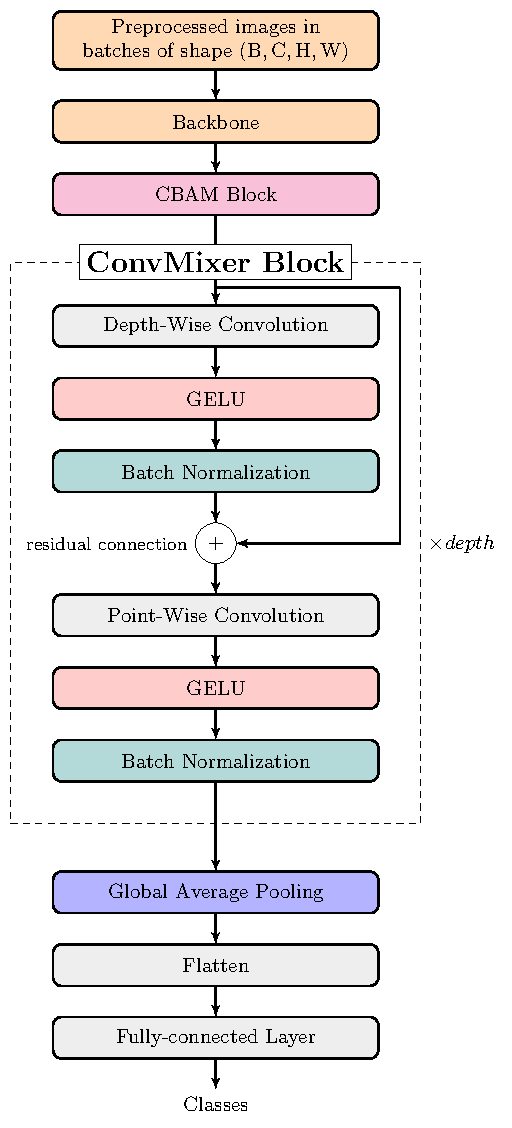
\includegraphics[width=0.8\textwidth]{model.pdf}
         \end{center}
    \end{column}
    \end{columns}
    \end{frame}

    \begin{frame}{Depthwise 及 Pointwise 卷积}
    \begin{columns}
        \begin{column}{0.5\textwidth}
            \begin{itemize}
                \item 将一次卷积运算拆分成两次独立的操作;
                \item Depthwise 卷积对每个通道使用不同的卷积核;
                \item Pointwise 卷积在每一个点上对通道进行卷积;
            \end{itemize}
        \end{column}
        \begin{column}{0.5\textwidth}
            \begin{center}
                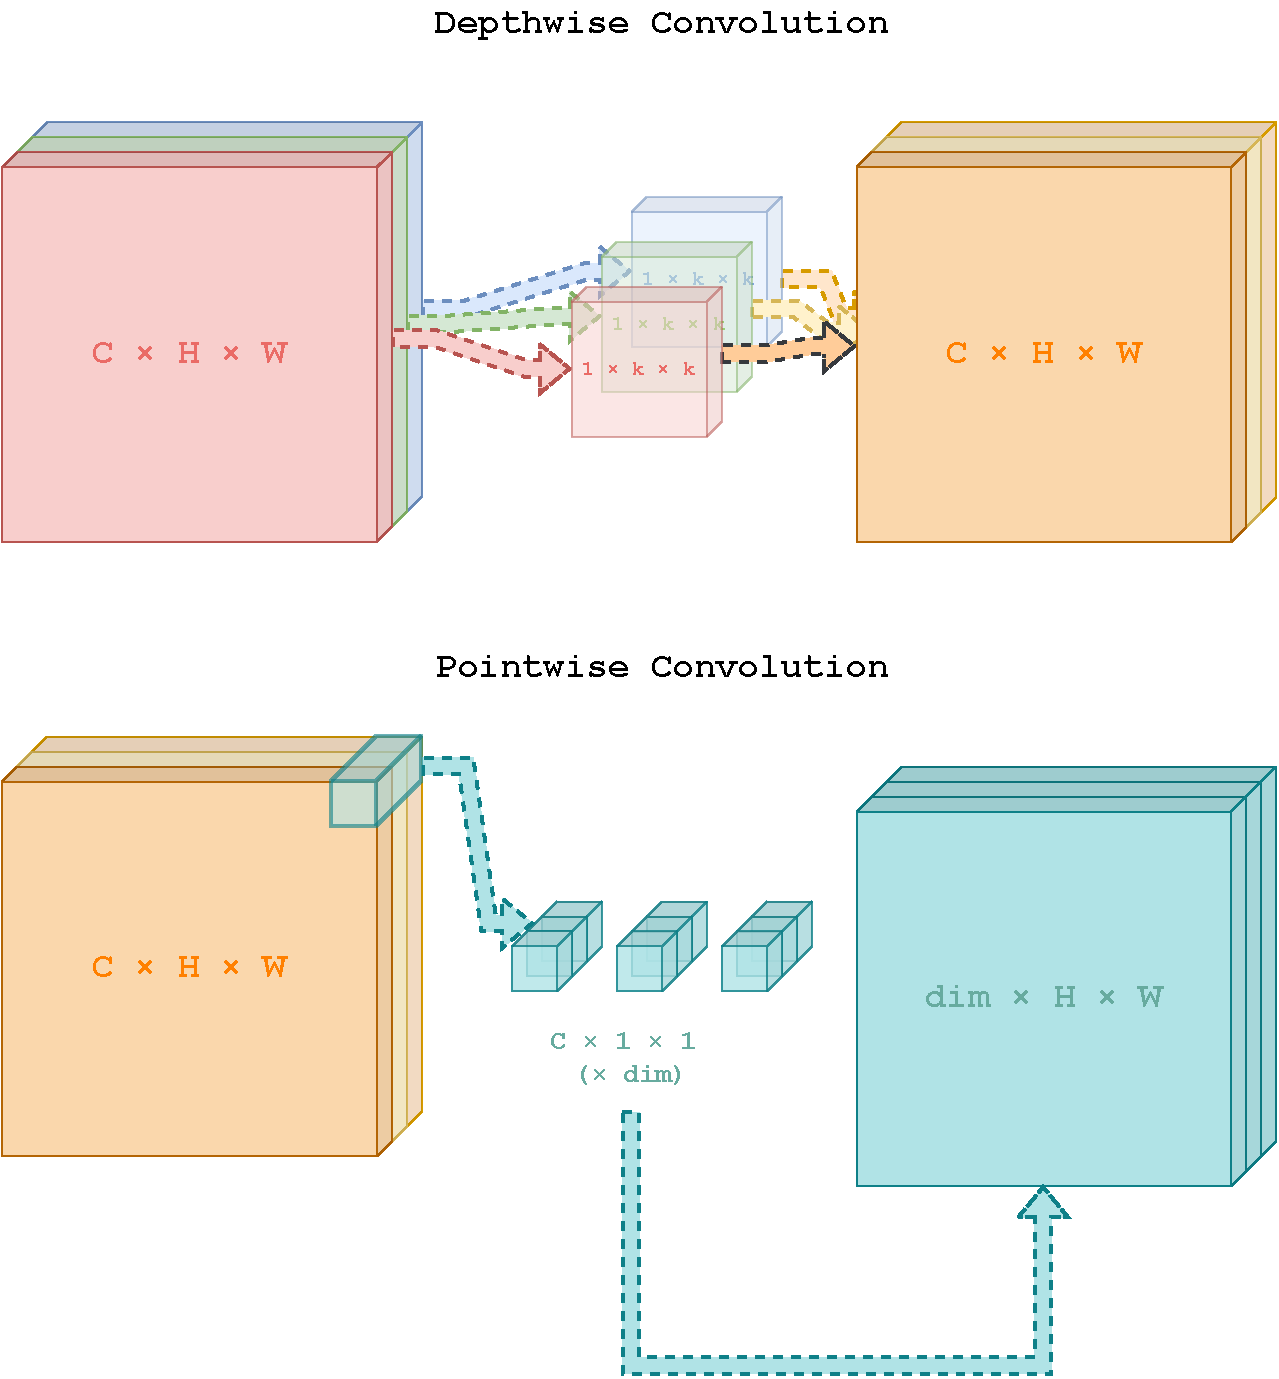
\includegraphics[width=0.85\textwidth]{depth_point_wise_conv.pdf}
            \end{center}
        \end{column}
    \end{columns}
        
    \end{frame}

    \begin{frame}{Backbones}
            \begin{itemize}
                \item Patch Embedding
                    \begin{itemize}
                    \item ConvMixer 原网络
                    \item 将输入进行分块卷积(步长与卷积核大小均为 $p$)
                    \end{itemize}
                \item ConvNeXt
                    \begin{itemize}
                    \item 综合了过去各种网络中的优点
                    \item 具有良好的性能\cite{liu2022}
                    \item 实验中使用冻结参数连接 CBAM 和 ConvMixer、不冻结参数连接 CBAM 和 ConvMixer、不冻结参数更换全连接层这三种方式进行训练并进行了对比。
                    \end{itemize}
                \item EfficientNet
                    \begin{itemize}
                    \item 较少的参数量和较快的速度\cite{tan2019}
                    \end{itemize}
                \item DenseNet
                    \begin{itemize}
                    \item 将每一层的处理结果连接(Concatenate)\cite{huang2016}
                    \end{itemize}
            \end{itemize}
        
    \end{frame}

    \begin{frame}{GAB+CAB}
    \begin{columns}
        
        \begin{column}{0.5\textwidth}
            Global Attention 过程可以表示如下
            $$
                \begin{aligned}
                w_1 &=\sigma(\mathsf{Conv}(\mathsf{AvgPool}(x_0)))\\
                x_1 &= w_1 \otimes x_0\\
                w_2 &=\sigma(\mathsf{AvgPool_{channel}}(x_1))\\
                x_2 &= w_2 \otimes x_1
                \end{aligned}
            $$
        \end{column}
        \begin{column}{0.5\textwidth}
            Category Attention 模块过程大致如下
            \begin{enumerate}
                \item 将通道数通过卷积增广到 $k\times L$,其中 $L$ 表示类别数量,通过池化得到每一类的权重;
                \item 在改变维数后对 $k$ 所在维度池化
                \item 将两种操作结果对应元素相乘并在通道维数上池化得到权重
                \item 权重与 Global Attention 结果相乘得到 CAB 的处理结果。
            \end{enumerate}
            最后通过池化、Flatten 和全连接层得到分类结果。实验中根据 CABNet 论文中的实验结果,取 $k=5$。
        \end{column}
    \end{columns}
    \end{frame}

\section{实验}

    \begin{frame}{训练设置}
        \begin{itemize}
            \item AdamW 优化器
            \item Label Smoothing + CrossEntropy 作为损失函数
            \item 学习率下降
        \end{itemize}
    \end{frame}

    \begin{frame}{评估指标}
        \begin{itemize}
            \item Accuracy
            \item Kappa\cite{cohen1960}
                \begin{itemize}
                    \item 令 $f_{ij}$ 表示混淆矩阵中第 $i$ 行第 $j$ 列,Kappa 系数的定义如下:
                        $$
                        \begin{aligned}
                        \mathrm{Kappa} &= \frac{p_o-p_e}{1-p_e}\\
                        p_o &= \frac{1}{n}\sum_i^k f_{ii}\\
                        p_e &= \frac{1}{n^2}\sum_i^k f_{i\cdot}\times f_{\cdot i}\\
                        \end{aligned}
                        $$
                    \item 在样本不均衡的情况下考虑小样本的分类情况
                    \item 更好地评估分类精度
                \end{itemize}
        \end{itemize}
    \end{frame}

    
    \begin{frame}[allowframebreaks]
        \frametitle{实验结果}
        \centering
        \resizebox{\linewidth}{!}{\begin{tabular}{lclclllc}
        \toprule
        Backbone        & Parameters     & Classification Net & Depth & Accuracy        & Kappa           & Image          & Batch Size \\
        \midrule
        Patch-Embedding & not pretrained & CBAM + ConvMixer   & 8     & 0.6911          & 0.4618          & 480$\times$480 & 128        \\
        ConvNeXt        & unfreezed      & FC                 & 8     & \textbf{0.8399} & 0.\textbf{7227} & 480$\times$480 & 32         \\
        ConvNeXt        & unfreezed      & CBAM + ConvMixer   & 4     & \textbf{0.8399} & 0.7218          & 480$\times$480 & 32         \\
        ConvNeXt        & unfreezed      & GAB + CAB          & -     &  0.8284         & 0.7001          & 480$\times$480 & 32\\
        ConvNeXt        & freezed        & CBAM + ConvMixer   & 8     & 0.7526          & 0.5599          & 480$\times$480 & 128        \\
        ConvNeXt        & freezed        & GAB + CAB          & -     &  0.7023         & 0.4717          & 480$\times$480 & 128        \\
        EfficientNet    & unfreezed      & CBAM + ConvMixer   & 8     & 0.7571          & 0.5725          & 480$\times$480 & 32         \\
        DenseNet        & unfreezed      & CBAM + ConvMixer   & 8     & 0.7840          & 0.6190          & 480$\times$480 & 32         \\
        \bottomrule
    \end{tabular}}
    
    \centering
    \includegraphics[width=0.8\linewidth]{acc.pdf}
        
    \end{frame}
    
    \begin{frame}{分析}
    \begin{itemize}
        \item 从零开始训练的使用 Patch Embedding 的网络效果较差
        \item 冻结了参数的 ConvNeXt 加上后续网络和未冻结参数的 EfficientNet 和 DenseNet 加上后续网络结果相差不大
        \item 未冻结参数的 ConvNeXt 后接 CBAM+ConvMixer 训练时比纯全连接层略好,但测试结果相差并不大。
        \item 从 Kappa 结果根据 Landis 和 Koch 等人提出的标准\cite{landis1977} 来看,ConvNeXt 不冻结参数训练得到的分类结果具有高度的一致性(Substantial)
        \item ConvNeXt 作为特征提取器后使用 FC, CBAM+ConvMixer 以及 CABNet 都能够取得较好的结果。
    \end{itemize}
    \end{frame}

    \begin{frame}{CBAM 与 CABNet 注意力机制对比}
    \begin{columns}
        \begin{column}{0.4\textwidth}
              图为以 ConvNeXt 为 Backbone 的网络下使用 CBAM + ConvMixer 和 CABNet 中注意力机制得到的结果。可以直观地发现 GAB+CAB 对原始图片中特征的刻画的确是更加准确的。
        \end{column}
        \begin{column}{0.6\textwidth}
                    
            \begin{figure}[H]
                \centering
                \begin{subfigure}[b]{0.2\textwidth}
                    \raggedleft
                    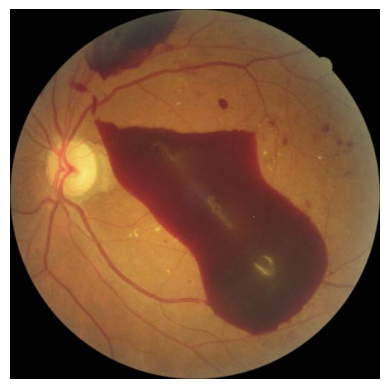
\includegraphics[width=\textwidth]{image-1.png}
                \end{subfigure}
                \hspace{2mm}
                \begin{subfigure}[b]{0.2\textwidth}
                    \centering
                    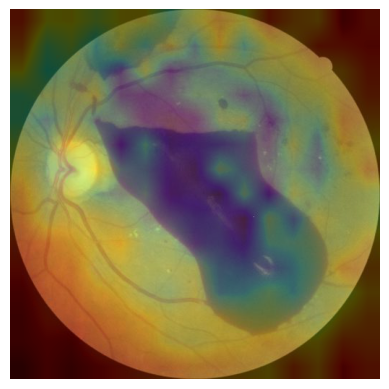
\includegraphics[width=\textwidth]{cbam-heatmap-1.png}
                \end{subfigure}
                \hspace{2mm}
                \begin{subfigure}[b]{0.2\textwidth}
                    \raggedright
                    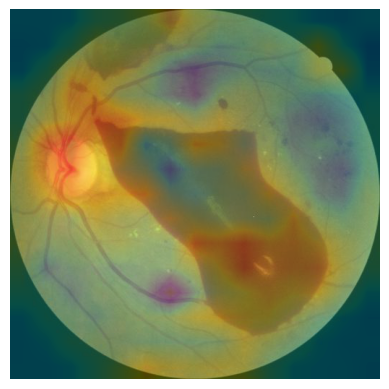
\includegraphics[width=\textwidth]{cabnet-heatmap-1.png}
                \end{subfigure} \\
                \vspace{2mm}
                \begin{subfigure}[b]{0.2\textwidth}
                    \raggedleft
                    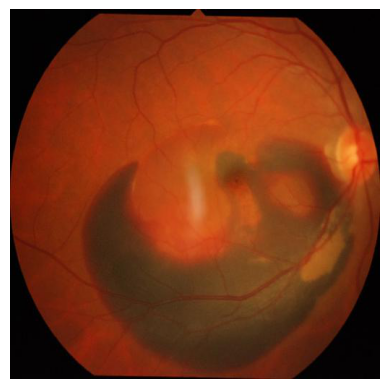
\includegraphics[width=\textwidth]{image-2.png}
                \end{subfigure}
                \hspace{2mm}
                \begin{subfigure}[b]{0.2\textwidth}
                    \centering
                    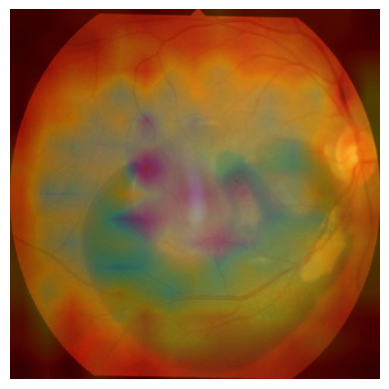
\includegraphics[width=\textwidth]{cbam-heatmap-2.png}
                \end{subfigure}
                \hspace{2mm}
                \begin{subfigure}[b]{0.2\textwidth}
                    \raggedright
                    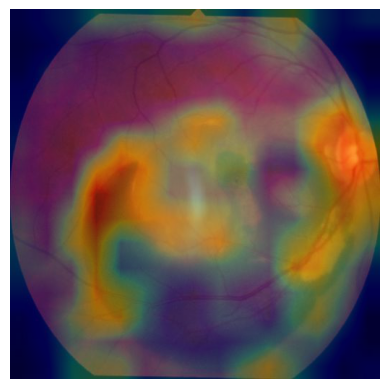
\includegraphics[width=\textwidth]{cabnet-heatmap-2.png}
                \end{subfigure} \\
                \vspace{2mm}
                \begin{subfigure}[b]{0.2\textwidth}
                    \raggedleft
                    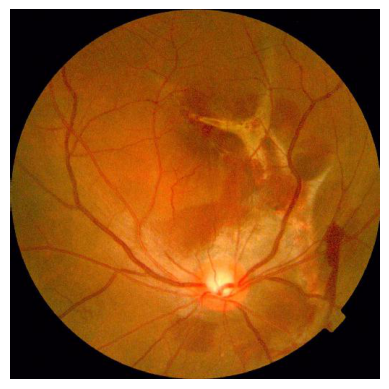
\includegraphics[width=\textwidth]{image-3.png}
                    \caption{原始图片}
                \end{subfigure}
                \hspace{2mm}
                \begin{subfigure}[b]{0.2\textwidth}
                    \centering
                    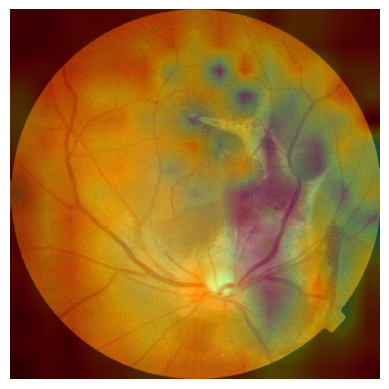
\includegraphics[width=\textwidth]{cbam-heatmap-3.png}
                    \caption{CBAM}
                \end{subfigure}
                \hspace{2mm}
                \begin{subfigure}[b]{0.2\textwidth}
                    \raggedright
                    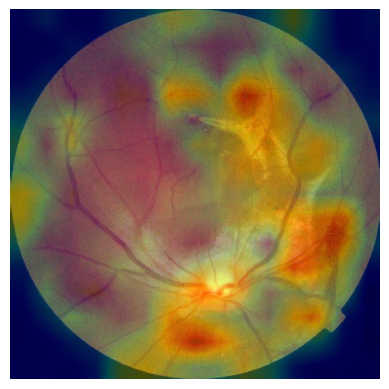
\includegraphics[width=\textwidth]{cabnet-heatmap-3.png}
                    \caption{GAB+CAB}
                \end{subfigure}
            \end{figure}
        \end{column}
    \end{columns}

        
    \end{frame}

    \begin{frame}{混淆矩阵}
    \begin{columns}
        \begin{column}{0.5\textwidth}
              使用 ConvNext+CBAM+ConvMixer 模型在 test 集上得到的混淆矩阵如右图。
        \end{column}
        \begin{column}{0.5\textwidth}
            \centering
            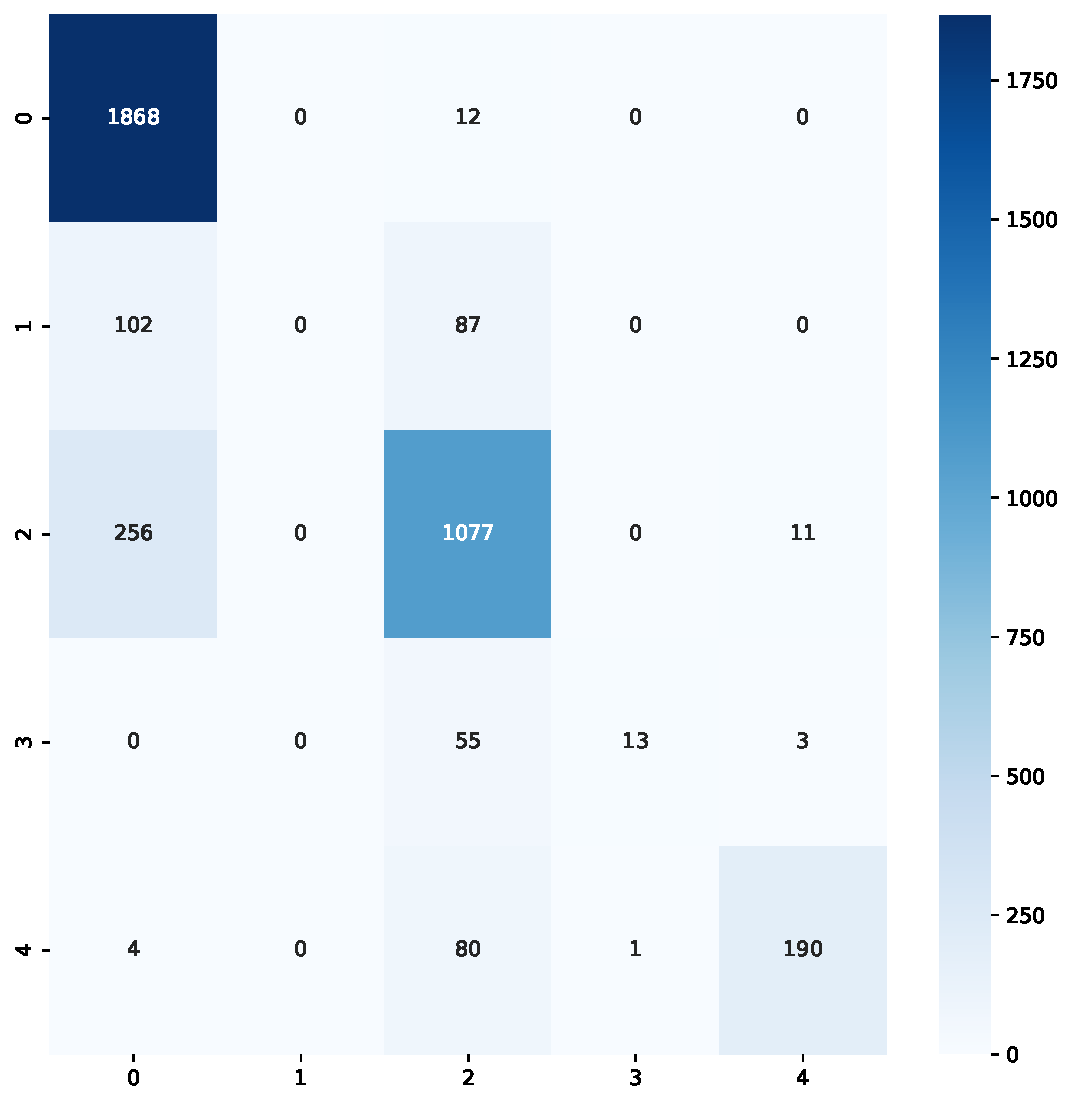
\includegraphics[width=0.8\textwidth]{confusion_matrix.pdf}
        \end{column}
    \end{columns}

        
    \end{frame}

\section*{参考文献}
\begin{frame}[allowframebreaks]
    \linespread{1.1}
    \frametitle{参考文献}
    \small
    \nocite{*}
    \bibliographystyle{plain}
    \bibliography{references}
\end{frame}


\section*{致谢}  
\begin{frame}
\centering
\let\thefootnote\relax\footnotetext{实验报告及演示文稿使用 Overleaf 及 \LaTeX 编写}
\let\thefootnote\relax\footnotetext{报告及演示文稿中的示意图使用 \LaTeX, TikZ 以及 draw.io 完成}
\let\thefootnote\relax\footnotetext{}

\textcolor{myNewColorA}{\Huge{\centerline{谢谢!}}}
\end{frame}


\end{document}



